   
   \section{Interactions}

   \begin{frame}
      \frametitle{Interactions}
      \begin{center}
      \Huge{Interactions}
      \end{center}
   \end{frame}
   
   \begin{frame}
      \frametitle{Interactions}
      \begin{itemize}
         \item TrickHLA supports interactions that are either Timestamp Order
         (TSO) or Receive Order (RO).
         \item Configuring TrickHLA interactions involves three steps:
         \begin{itemize}
            \item Step 1: Extend the \texttt{TrickHLA::InteractionHandler} class
            and implement the virtual \texttt{receive\_interaction()} function.
            \item Step 2: Add your interaction-handler object to each simulation
            object that needs to process interactions in your \texttt{S\_define} file.
            \item Step 3: Configure the interaction-handlers in the \texttt{input.py} file.
            \item Step 4: Send interactions at specified times using the
            \texttt{input.py} file or programmatically within your simulation.
         \end{itemize}
      \end{itemize}
   \end{frame}
   
   \begin{frame}[fragile]
      \frametitle{Interactions}
      \framesubtitle{Step 1: Extend the \texttt{TrickHLA::InteractionHandler} Class}
      \begin{itemize}
         \item Step 1: This is a snippet of the base class from
         \texttt{TrickHLA::InteractionHandler.hh} that you must extend and then
         implement the virtual \texttt{receive\_interaction()} function:
      \end{itemize}
\begin{Verbatim}[frame=single, fontsize=\scriptsize]
class TrickHLA::InteractionHandler
{
  ...
  public:
   ...
   virtual void initialize_callback( TrickHLAInteraction * inter );

   bool send_interaction();                   // Receive Order
   bool send_interaction( double send_time ); // Timestamp Order

   // This is a virtual function and must be defined by a full class.
   virtual void receive_interaction();
   ...
};
\end{Verbatim}
   \end{frame}

   \begin{frame}[fragile]
      \frametitle{Interactions}
      \framesubtitle{Step 1: Extend the \texttt{TrickHLA::InteractionHandler} - \texttt{SineInteractionHandler.hh}}
      \begin{itemize}
         \item Extended in \texttt{SineInteractionHandler.hh}:
      \end{itemize}
      \vspace{0.2cm}
\begin{Verbatim}[frame=single, fontsize=\tiny]
#include "TrickHLA/include/TrickHLAInteractionHandler.hh"

class SineInteractionHandler : public TrickHLAInteractionHandler
{
  ...
  public:
   ...
   void send_sine_interaction( double sim_time );

   virtual void receive_interaction();

   char *   name;    // -- Example of a unique name to identify the interaction handler.
   char *   message; // -- Example of a static array of strings.

  protected:
   double   time;        // s  Example of floating-point data.
   int      year;        // -- Example of integer data.
   int      send_cnt;    // -- The number of times an interaction is sent.
   int      receive_cnt; // -- The number of times an interaction was received.};
};
\end{Verbatim}
   \end{frame}

   \begin{frame}[fragile]
      \frametitle{Interactions}
      \framesubtitle{Step 1: Extend the \texttt{TrickHLA::InteractionHandler} - \texttt{SineInteractionHandler.cpp}}
      \begin{itemize}
         \item Extended in \texttt{SineInteractionHandler.cpp}:
      \end{itemize}
\begin{Verbatim}[frame=single, fontsize=\tiny]
void SineInteractionHandler::send_sine_interaction( // RETURN: -- None.
   double sim_time)        // IN: s Current simulation time.
{
   time = sim_time;    // Update the time with the simulation time.
   ostringstream msg;  // Create a message to send
   msg << "Interaction from:\"" << ((name != NULL) ? name : "Unknown") << "\" "
       << "Send-count:" << (send_cnt + 1);
   if ( ( message != NULL ) && TMM_is_alloced( message ) ) {
      TMM_delete_var_a( message );
   }
   message = TMM_strdup( (char *)msg.str().c_str() );

   double lookahead_time = get_fed_lookahead().getDoubleTime();
   double timestamp = time + lookahead_time;
   // Notify the parent interaction handler to send the interaction using
   // Timestamp Order (TSO) at the current simulation time plus the lookahead_time.
   bool was_sent = this->TrickHLAInteractionHandler::send_interaction( timestamp );
   if ( was_sent ) {
      cout << "++++SENDING++++ SineInteractionHandler::send_sine_interaction() << endl
           << "  name:'" << ((name != NULL) ? name : "NULL") << "'" << endl
           << "  message:'" << ((message != NULL) ? message : "NULL") << "'" << endl
           << "  timestamp:" << timestamp;
      send_cnt++; // Update send count, just used for the message in this example
   } else {
      cout << "+-+-NOT SENT-+-+ SineInteractionHandler::send_sine_interaction()" << endl         
}
\end{Verbatim}
   \end{frame}

   \begin{frame}[fragile]
      \frametitle{Interactions}
      \framesubtitle{Step 1: Extend the \texttt{TrickHLA::InteractionHandler} - \texttt{SineInteractionHandler.cpp}}
      \begin{itemize}
         \item Extended in \texttt{SineInteractionHandler.cpp} (Continued):
      \end{itemize}
      \vspace{0.2cm}
\begin{Verbatim}[frame=single, fontsize=\tiny]
void SineInteractionHandler::receive_interaction() // RETURN: -- None.
{
   receive_cnt++;
   double sim_time = exec_get_sim_time();

   cout << "++++RECEIVING++++ SineInteractionHandler::receive_interaction()" << endl
        << "  name:'" << ((name != NULL) ? name : "NULL") << "'" << endl
        << "  message:'" << ((message != NULL) ? message : "NULL") << "'" << endl
        << "  message length:" << ((message != NULL) ? strlen(message) : 0) << endl
        << "  sim_time:" << sim_time << endl
        << "  time:" << time << endl
        << "  year:" << year << endl
        << "  receive_cnt:" << receive_cnt << endl;
}
\end{Verbatim}
   \end{frame}

   \begin{frame}[fragile]
      \frametitle{Interactions}
      \framesubtitle{Step 2: Add Interaction-handler Object to \texttt{S\_define}}
      \begin{itemize}
         \item Step 2: In the \texttt{S\_define} file add your interaction-handler
         object to each simulation object that needs to process interactions.  
      \end{itemize}
\begin{Verbatim}[frame=single, fontsize=\tiny]
   class ASimObject : public Trick::SimObject {

      SineData     sim_data;
      SinePacking            packing;
      SineInteractionHandler interaction_handler;

      ASimObject() {
        P50 ("initialization") packing.initialize( &sim_data );
        ...
      }
   };

   class PSimObject : public Trick::SimObject {
      ...
      SineData     sim_data;
      SinePacking            packing;
      SineInteractionHandler interaction_handler;

      PSimObject() {
        P50 ("initialization") packing.initialize( &sim_data );
        ...
      }
   };
\end{Verbatim}
   \end{frame}

   \begin{frame}[fragile]
      \frametitle{Interactions}
      \framesubtitle{Step 3: Configure the interaction-handlers in the \texttt{input.py} file}
      \begin{itemize}
         \item Step 3: Example in the \texttt{RUN\_a\_side/input.py} file:
      \end{itemize}
\begin{Verbatim}[frame=single, fontsize=\tiny]
# We are taking advantage of the input file to specify a unique name for each handler
A.interaction_handler.name = "A-side: A.interaction_handler.name"
P.interaction_handler.name = "A-side: P.interaction_handler.name"

# Trick HLA Interactions and Parameters.
THLA.manager.inter_count  = 1
THLA.manager.interactions = trick.alloc_type( THLA.manager.inter_count, "TrickHLAInteraction" )

THLA.manager.interactions[0].FOM_name    = "Communication"
THLA.manager.interactions[0].publish     = True
THLA.manager.interactions[0].subscribe   = False
THLA.manager.interactions[0].handler     = A.interaction_handler
THLA.manager.interactions[0].param_count = 3
THLA.manager.interactions[0].parameters  = trick.alloc_type( THLA.manager.interactions[0].param_count,
                                           "TrickHLAParameter" )
THLA.manager.interactions[0].parameters[0].FOM_name   = "Message"
THLA.manager.interactions[0].parameters[0].trick_name = "A.interaction_handler.message"
THLA.manager.interactions[0].parameters[0].rti_encoding = trick.THLA_UNICODE_STRING

THLA.manager.interactions[0].parameters[1].FOM_name   = "time"
THLA.manager.interactions[0].parameters[1].trick_name = "A.interaction_handler.time"
THLA.manager.interactions[0].parameters[1].rti_encoding = trick.THLA_LITTLE_ENDIAN

THLA.manager.interactions[0].parameters[2].FOM_name   = "year"
THLA.manager.interactions[0].parameters[2].trick_name = "A.interaction_handler.year"
THLA.manager.interactions[0].parameters[2].rti_encoding = trick.THLA_LITTLE_ENDIAN
\end{Verbatim}
   \end{frame}

   \begin{frame}[fragile]
      \frametitle{Interactions}
      \framesubtitle{Step 3: Configure the interaction-handlers in the \texttt{input.py} file}
      \begin{itemize}
         \item Step 3: Example in the \texttt{RUN\_p\_side/input.py} file:
      \end{itemize}
\begin{Verbatim}[frame=single, fontsize=\tiny]
# We are taking advantage of the input file to specify a unique name for each handler
A.interaction_handler.name = P-side: A.interaction_handler.name"
P.interaction_handler.name = P-side: P.interaction_handler.name"

# TrickHLA Interactions and Parameters.
THLA.manager.inter_count  = 1
THLA.manager.interactions = trick.alloc_type( THLA.manager.inter_count, "TrickHLAInteraction" )

THLA.manager.interactions[0].FOM_name    = "Communication"
THLA.manager.interactions[0].publish     = False
THLA.manager.interactions[0].subscribe   = True
THLA.manager.interactions[0].handler     = P.interaction_handler
THLA.manager.interactions[0].param_count = 3
THLA.manager.interactions[0].parameters  = trick.alloc_type( THLA.manager.interactions[0].param_count,
                                           "TrickHLAParameter" )
THLA.manager.interactions[0].parameters[0].FOM_name   = "Message"
THLA.manager.interactions[0].parameters[0].trick_name = "P.interaction_handler.message"
THLA.manager.interactions[0].parameters[0].rti_encoding = trick.THLA_UNICODE_STRING

THLA.manager.interactions[0].parameters[1].FOM_name   = "time"
THLA.manager.interactions[0].parameters[1].trick_name = "P.interaction_handler.time"
THLA.manager.interactions[0].parameters[1].rti_encoding = trick.THLA_LITTLE_ENDIAN

THLA.manager.interactions[0].parameters[2].FOM_name   = "year"
THLA.manager.interactions[0].parameters[2].trick_name = "P.interaction_handler.year"
THLA.manager.interactions[0].parameters[2].rti_encoding = trick.THLA_LITTLE_ENDIAN
\end{Verbatim}
   \end{frame}

   \begin{frame}[fragile]
      \frametitle{Interactions}
      \framesubtitle{Step 4: Sending Interactions Using the Input File}
      \begin{itemize}
         \item Step 4: Add entries to the \texttt{input.py} file for when you
         want to send an interaction. For example, to send an interaction at
         time 10.0:
      \vspace{0.2cm}
\begin{Verbatim}[frame=single, fontsize=\tiny]
trick.add_read( 10.0, A.interaction_handler.send_sine_interaction(10.0) )
\end{Verbatim}
      \end{itemize}
   \end{frame}

   \begin{frame}
      \frametitle{Interactions}
      \framesubtitle{Sending and Receiving Interactions}
      \begin{itemize}
         \item Sending an interaction can be initiated three different ways:
         \begin{itemize}
            \item Programmatically, call one of the \texttt{send\_interaction()}
            functions inherited by your interaction-handler.
            \item As a job in your simulation specified in the \texttt{S\_define}
            file, which in turn calls \texttt{send\_interaction()} as above.
            \item As a job in your simulation called at a specific time from the
            \texttt{input.py} file, which in turn calls \texttt{send\_interaction()}
            as above.
         \end{itemize}
         \item TrickHLA will automatically process received interactions and
         call the \texttt{receive\_interaction()} function of the appropriate
         user defined interaction-handler.
         \item TrickHLA handles interactions in a thread-safe and Trick
         simulation environment job-safe way.
      \end{itemize}
   \end{frame}

   \begin{frame}
      \frametitle{Interactions}
      \framesubtitle{TrickHLA jobs in THLA.sm}
      \begin{figure}
      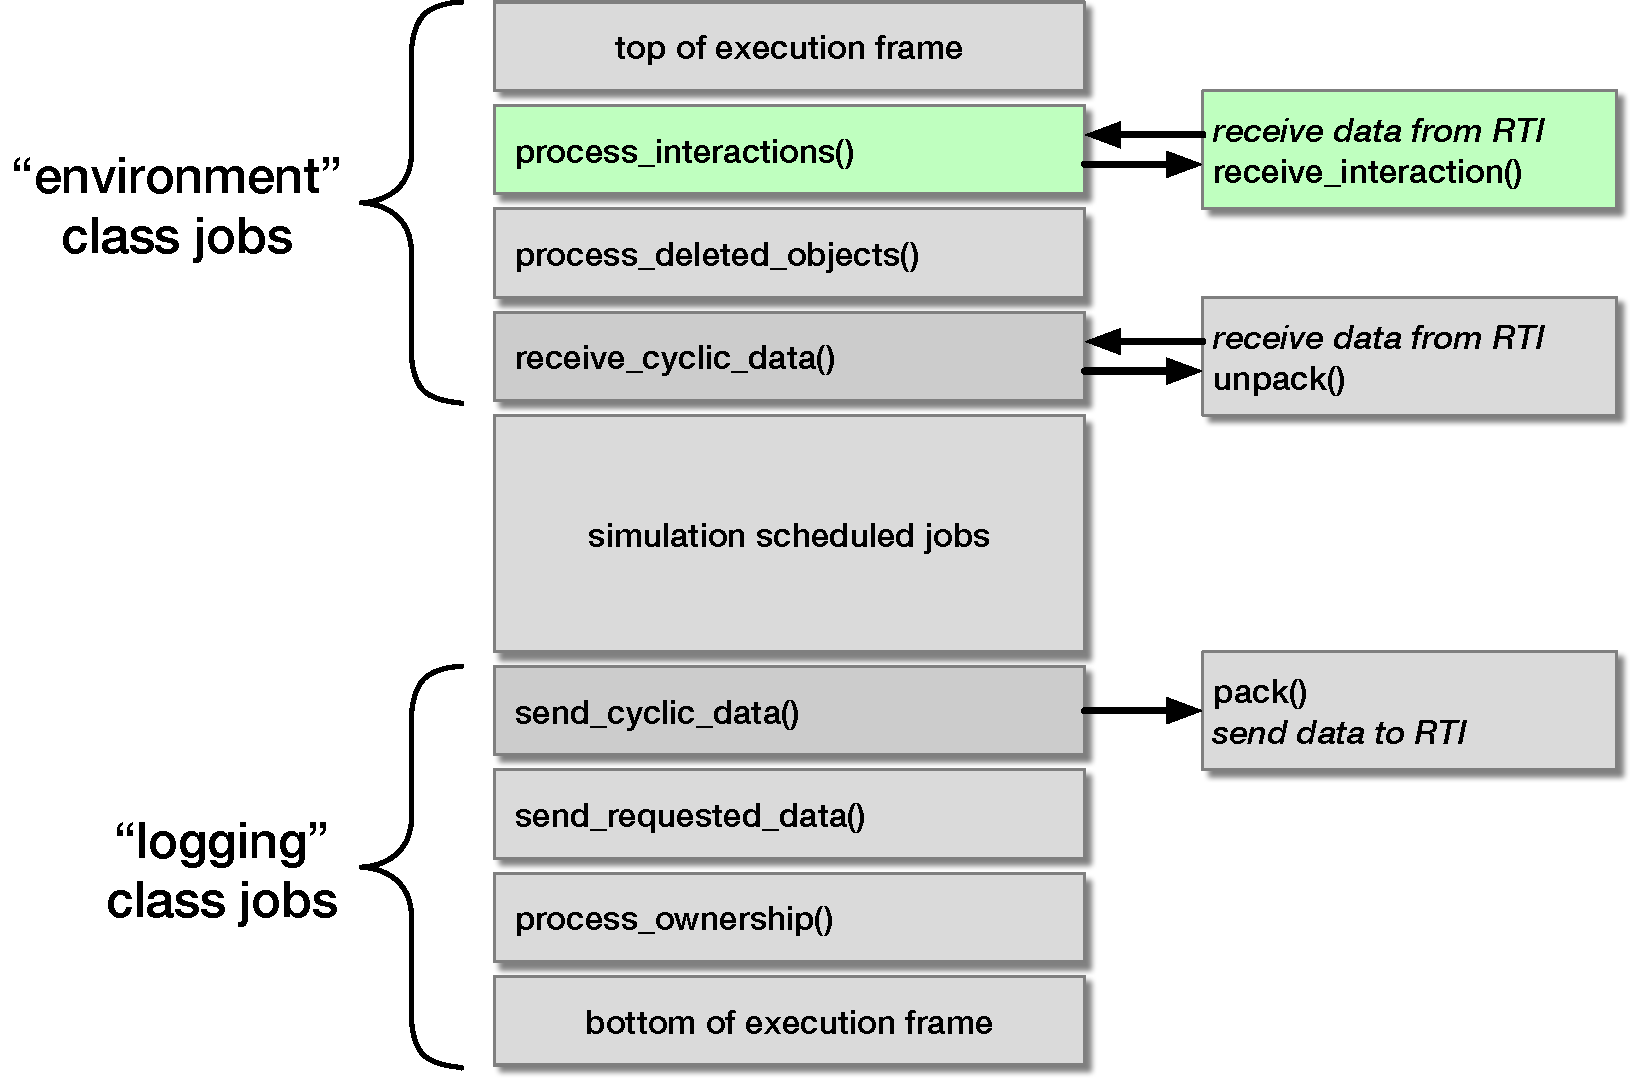
\includegraphics[scale=0.4]{TutorialTHLAInteractionJobs.pdf}
      \end{figure}
   \end{frame}
   
